\documentclass{report}
\usepackage[T1]{fontenc}
\usepackage[utf8]{inputenc}
\usepackage{lmodern}
%\usepackage{hyperref}
\usepackage[portuges,brazilian]{babel}
\usepackage{graphicx, subfigure}
\usepackage{textcomp}
\usepackage{fullpage}
\usepackage{wrapfig}
\usepackage{float}
\usepackage{listings}
\usepackage{amsmath}
\usepackage{amssymb}
\usepackage[margin=0.5in]{geometry}
\usepackage{pdfpages}

\begin{document}

\newcommand{\HRule}{\rule{\linewidth}{0.5mm}}
\newcommand{\tsize}[1]{(\frac{W}{L})_{#1}}
 

%%%%%%%%%%%%%%%%%%%%%%%%%% START TITLE PAGE %%%%%%%%%%%%%%%%%%%%%%%%5
\begin{titlepage}

\begin{center}


{\LARGE UNIVERSIDADE DE SÃO PAULO\\}
{\LARGE DEPARTAMENTO DE ENGENHARIA ELÉTRICA \\}
{\LARGE ESCOLA DE ENGENHARIA DE SÃO CARLOS\\[4cm]}

\textbf{\large SEL5755 - Sistemas Fuzzy}\\[1cm]
\textbf{\large Prof Dr. Ivan Nunes da Silva}\\[2cm]


% Title
\HRule \\[0.6cm]
{ \huge EPC 10\bfseries }\\[0.6cm]

\HRule \\[2cm]

% Author

\begin{center} \large
\end{center}

\begin{minipage}{\textwidth}
\begin{flushleft} \large
Isabela R. do Prado \textsc{Rossales}\\
6445435
\end{flushleft}
\end{minipage}

\vfill

% Bottom of the page
{\large São Carlos,\\ \today}

\end{center}

\end{titlepage}
%\listoffigures
%\begingroup
%\let\clearpage\relax
%\listoftables
%\endgroup
%%%%%%%%%%%%%%%%%%%%%%%%%% STOP TITLE PAGE %%%%%%%%%%%%%%%%%%%%%%%%5


\newpage


\includepdf[pages=1]{EPC10_Fuzzy.pdf}

\begin{figure}[h!]
\begin{center}
    \subfigure[Adição]{%
    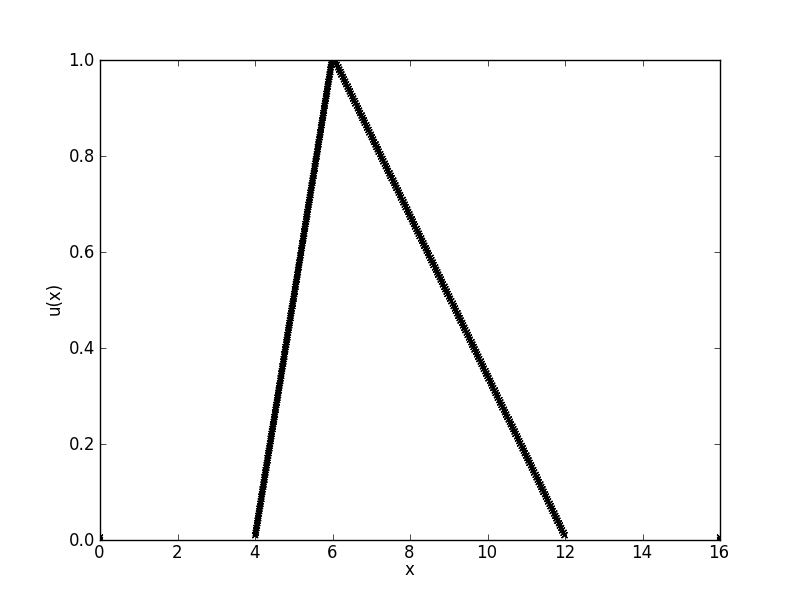
\includegraphics[width=0.15\textwidth]{graph0.png}
    }
    \subfigure[Subtração]{%
    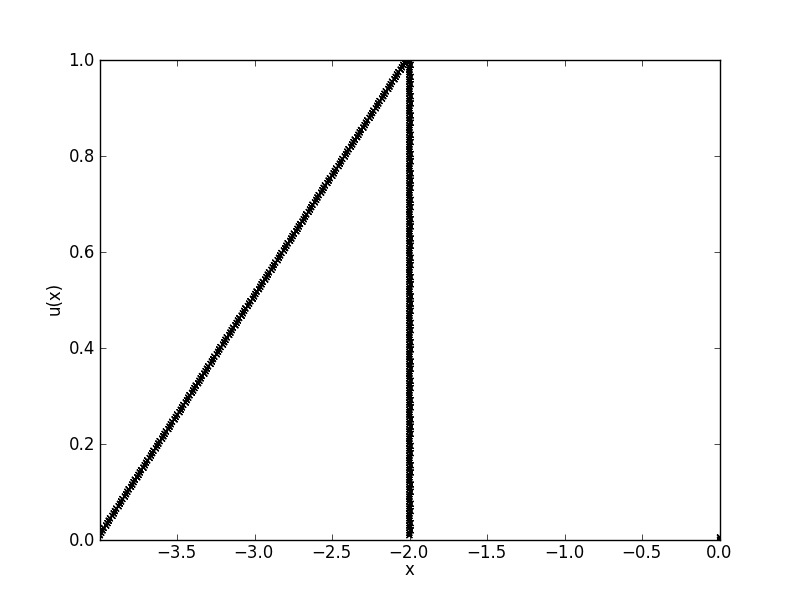
\includegraphics[width=0.15\textwidth]{graph1.png}
    }
    \subfigure[Multiplicação]{%
    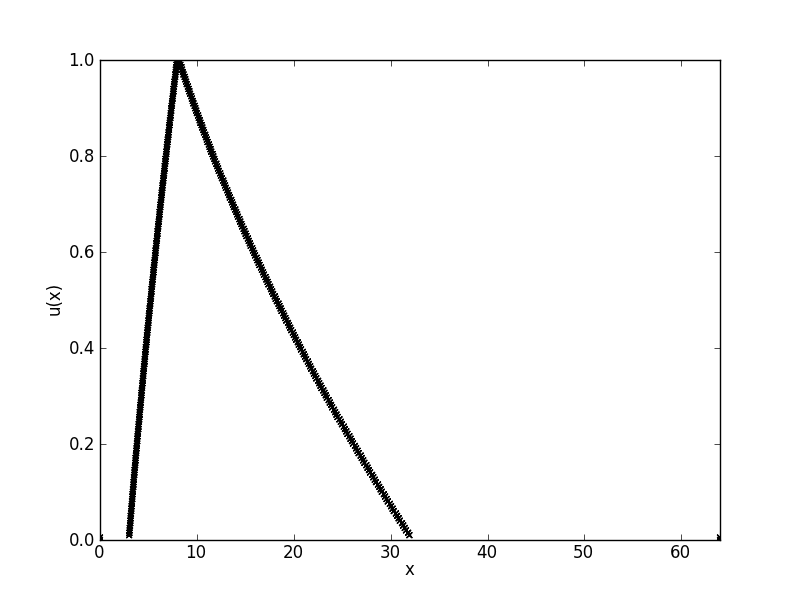
\includegraphics[width=0.15\textwidth]{graph2.png}
    }
    \subfigure[Divisão]{%
    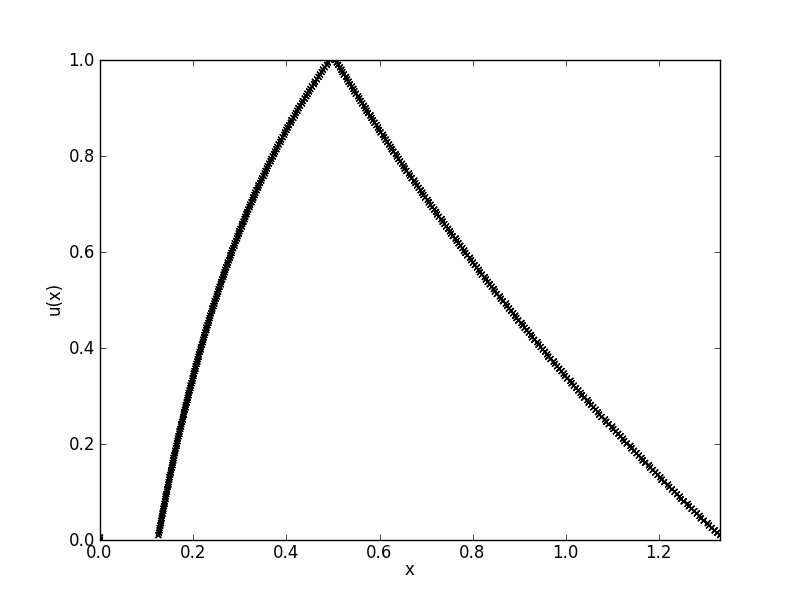
\includegraphics[width=0.15\textwidth]{graph3.png}
    }
    \subfigure[Mínimo]{%
    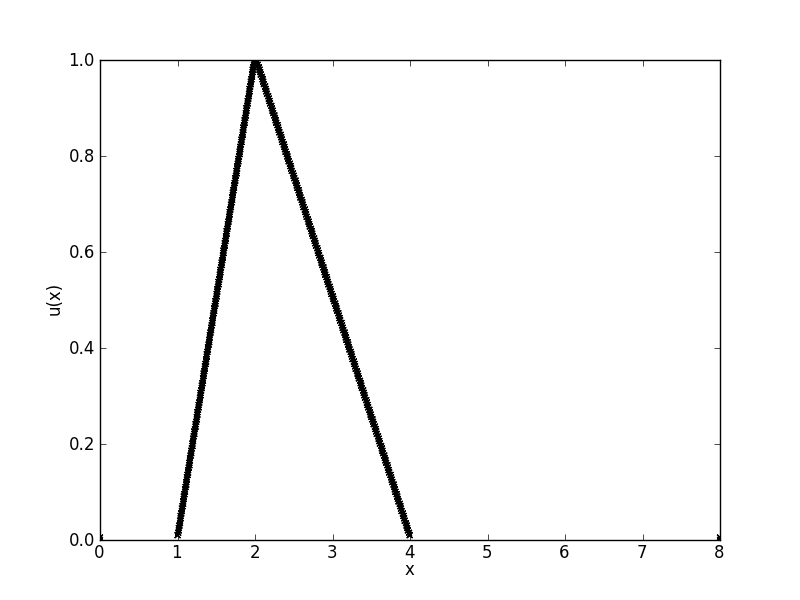
\includegraphics[width=0.15\textwidth]{graph4.png}
    }
    \subfigure[Máximo]{%
    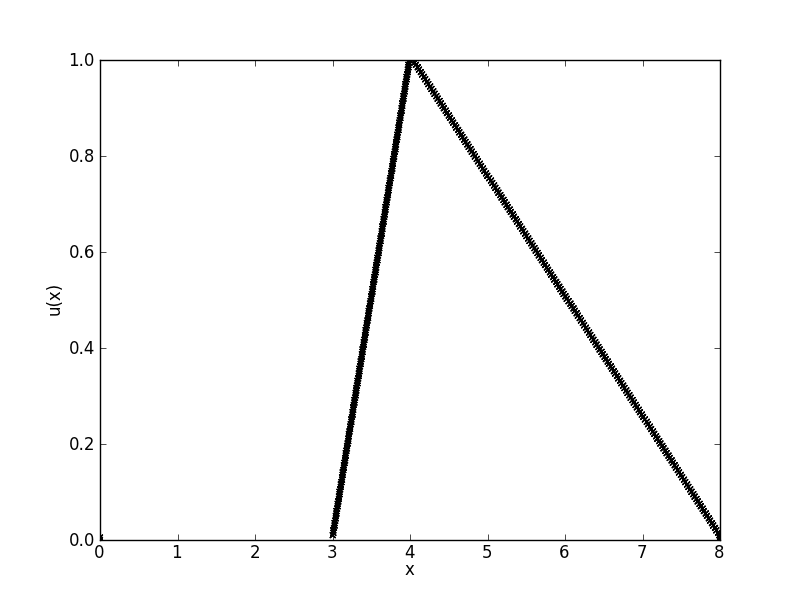
\includegraphics[width=0.15\textwidth]{graph5.png}
    }
\end{center}
\caption{$x_1$ = 2; $x_2$ = 4}
\end{figure}

\begin{figure}[h!]
\begin{center}
    \subfigure[Adição]{%
    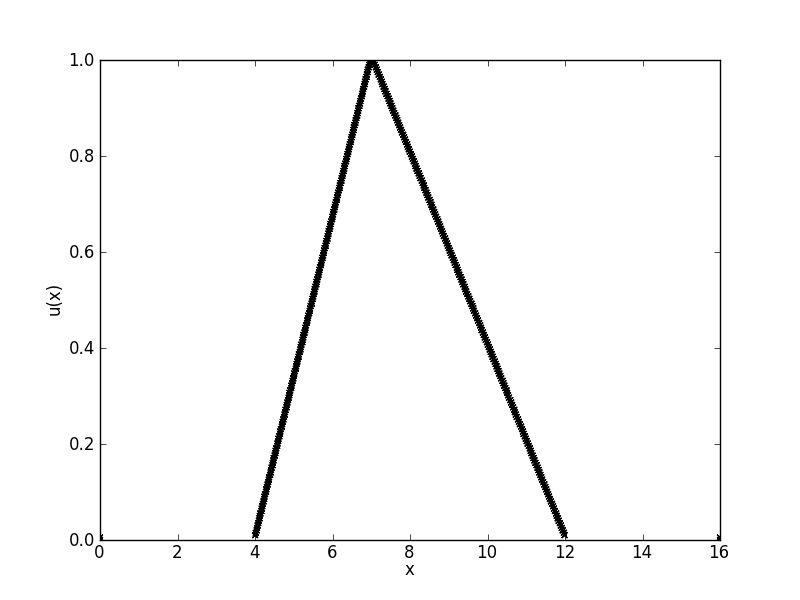
\includegraphics[width=0.15\textwidth]{graph6.png}
    }
    \subfigure[Subtração]{%
    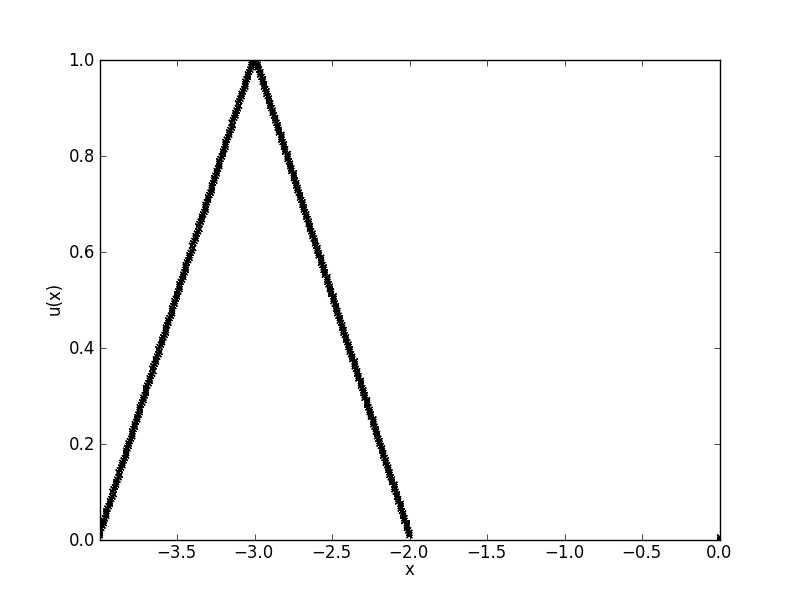
\includegraphics[width=0.15\textwidth]{graph7.png}
    }
    \subfigure[Multiplicação]{%
    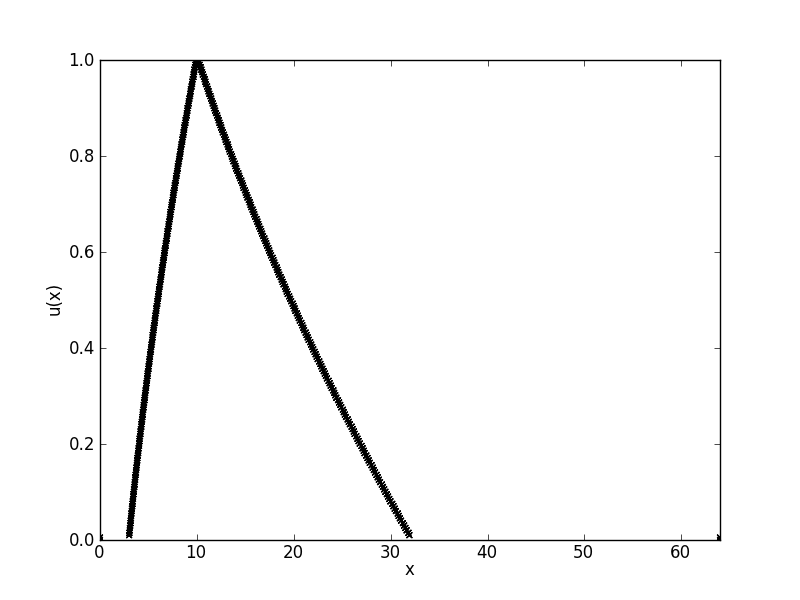
\includegraphics[width=0.15\textwidth]{graph8.png}
    }
    \subfigure[Divisão]{%
    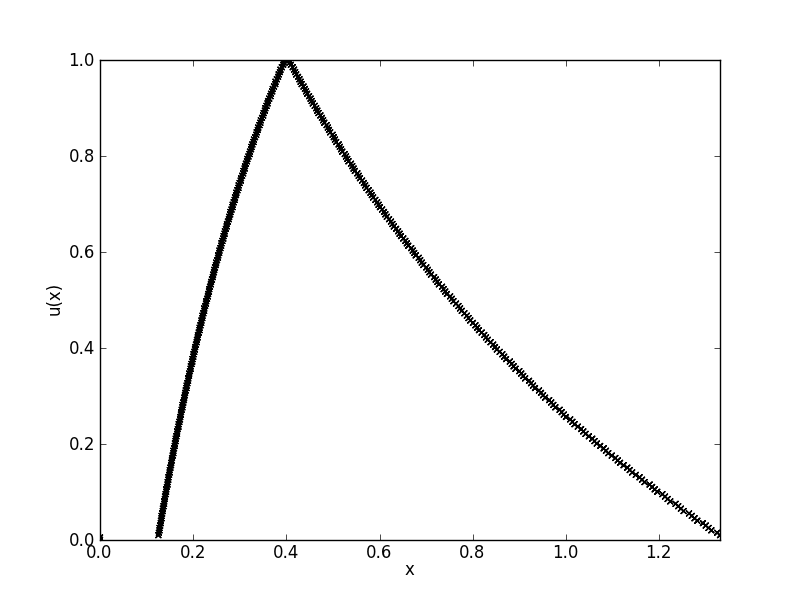
\includegraphics[width=0.15\textwidth]{graph9.png}
    }
    \subfigure[Mínimo]{%
    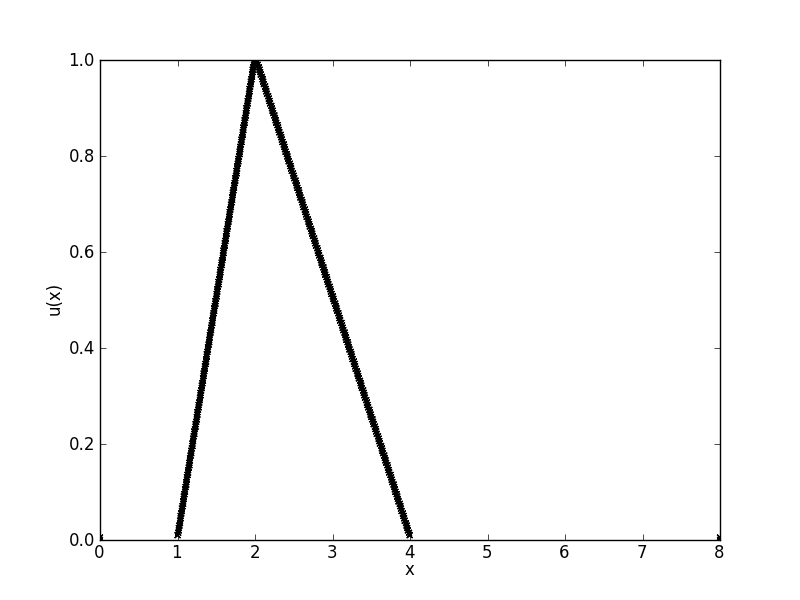
\includegraphics[width=0.15\textwidth]{graph10.png}
    }
    \subfigure[Máximo]{%
    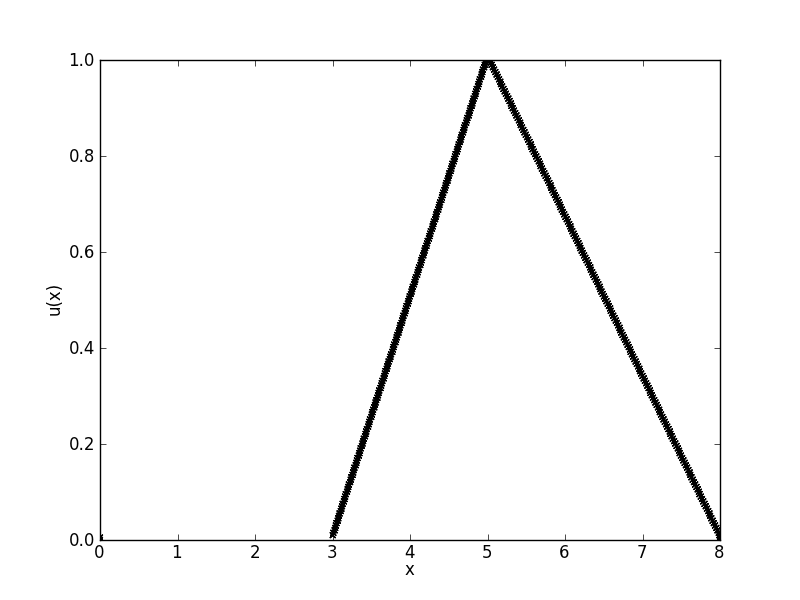
\includegraphics[width=0.15\textwidth]{graph11.png}
    }
\end{center}
\caption{$x_1$ = 2; $x_2$ = 5}
\end{figure}

\begin{figure}[h!]
\begin{center}
    \subfigure[Adição]{%
    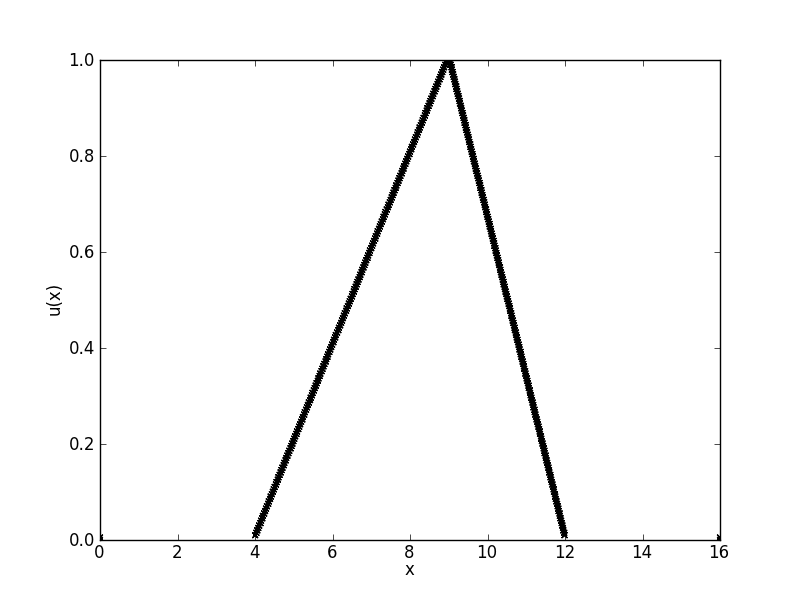
\includegraphics[width=0.15\textwidth]{graph12.png}
    }
    \subfigure[Subtração]{%
    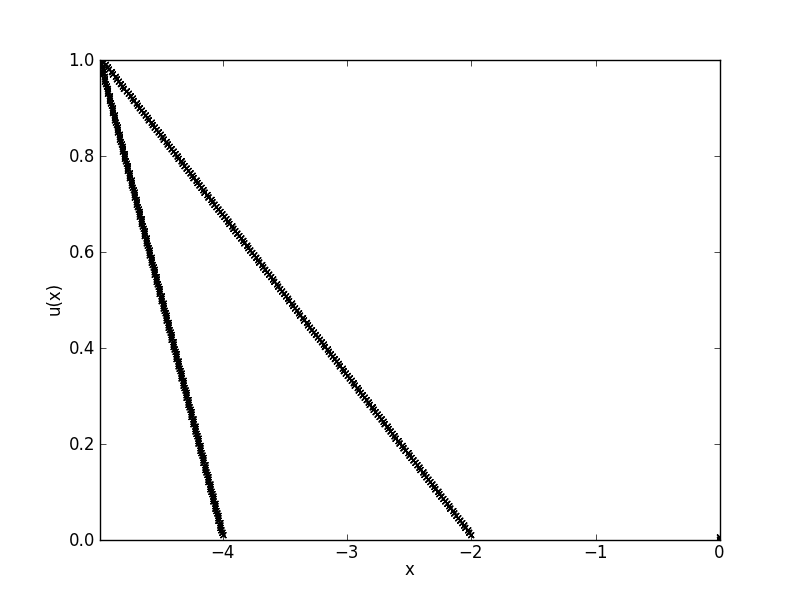
\includegraphics[width=0.15\textwidth]{graph13.png}
    }
    \subfigure[Multiplicação]{%
    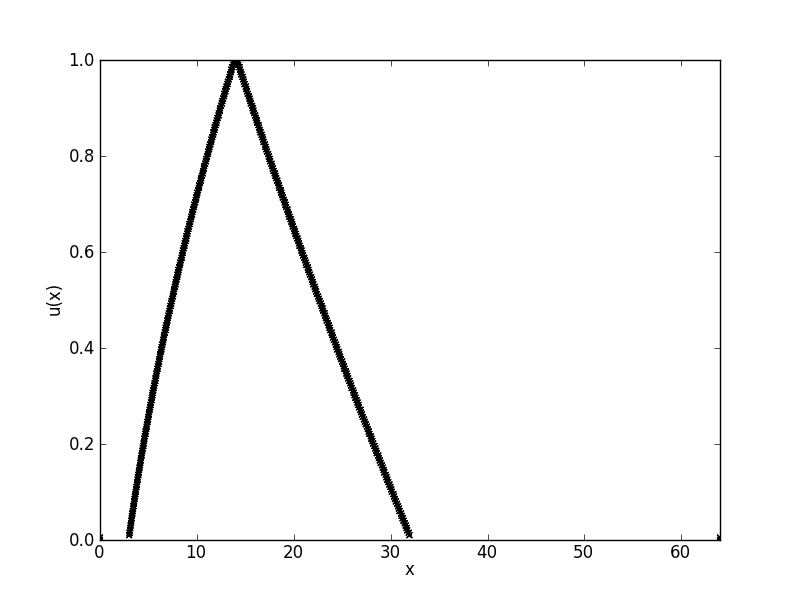
\includegraphics[width=0.15\textwidth]{graph14.png}
    }
    \subfigure[Divisão]{%
    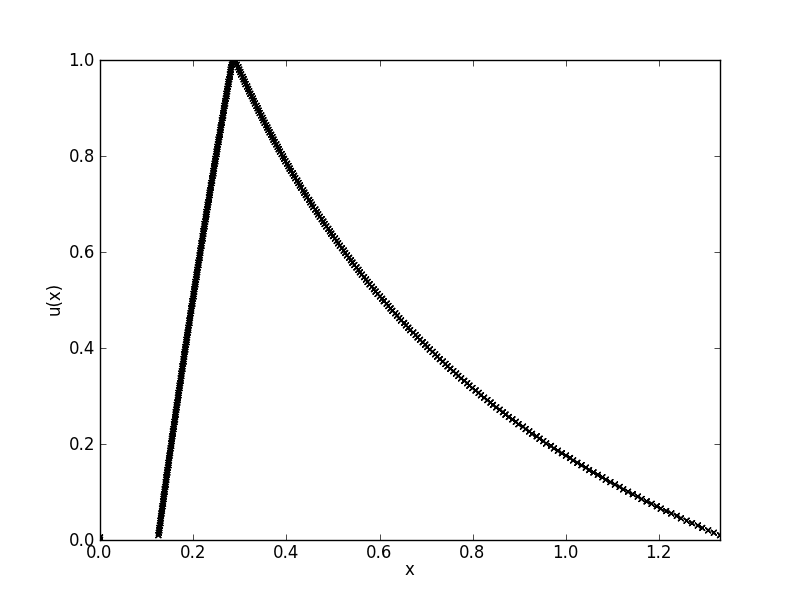
\includegraphics[width=0.15\textwidth]{graph15.png}
    }
    \subfigure[Mínimo]{%
    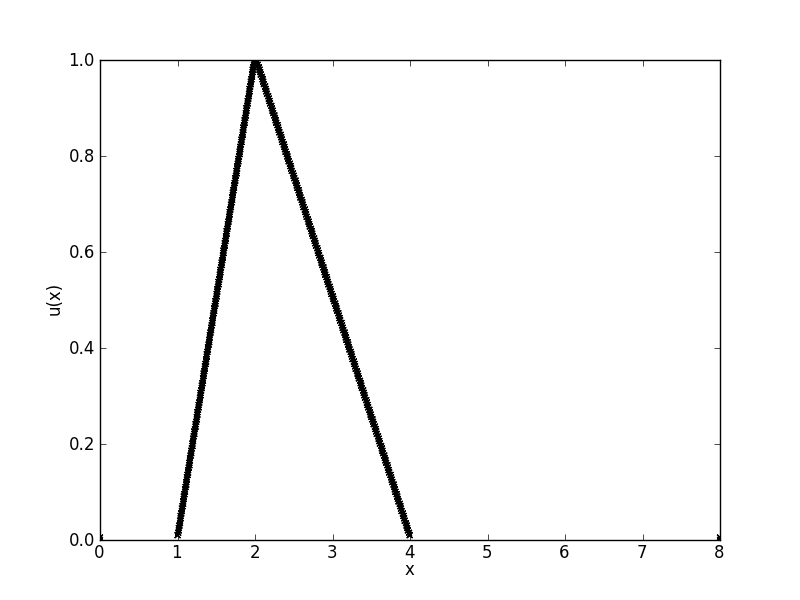
\includegraphics[width=0.15\textwidth]{graph16.png}
    }
    \subfigure[Máximo]{%
    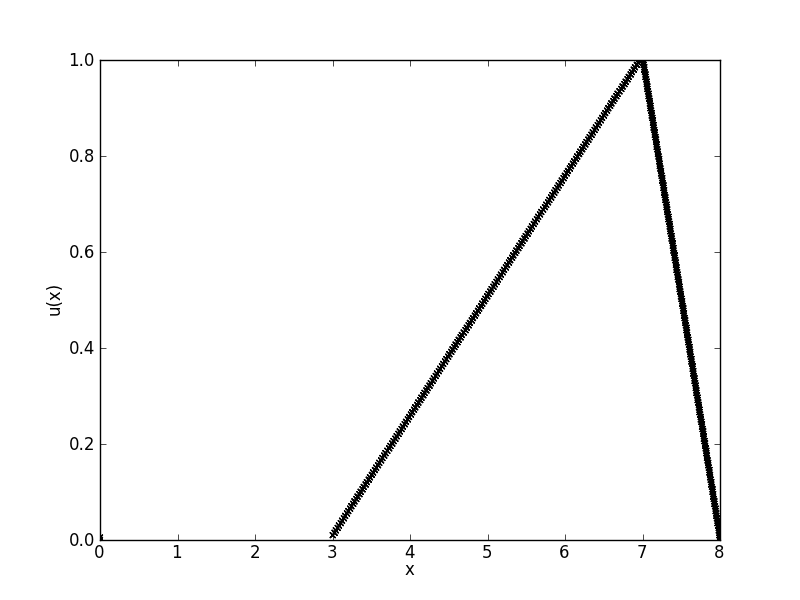
\includegraphics[width=0.15\textwidth]{graph17.png}
    }
\end{center}
\caption{$x_1$ = 2; $x_2$ = 7}
\end{figure}

\begin{figure}[h!]
\begin{center}
    \subfigure[Adição]{%
    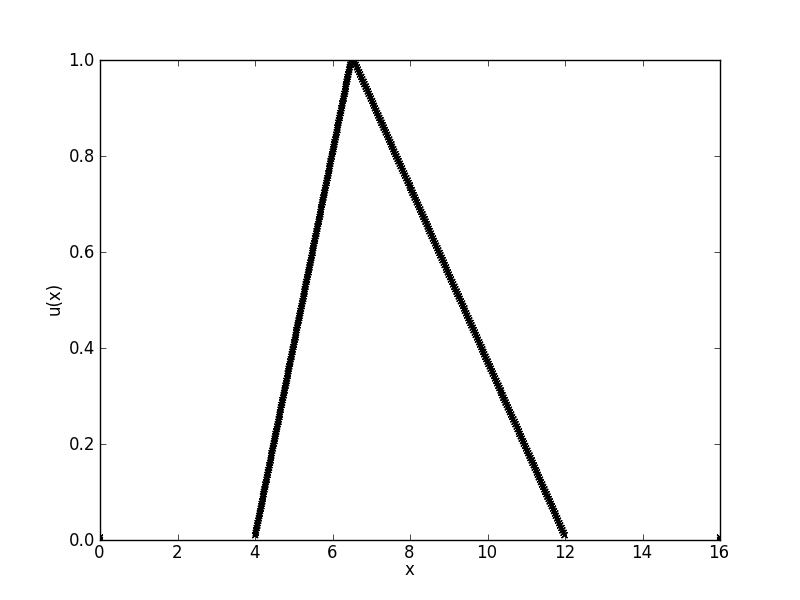
\includegraphics[width=0.15\textwidth]{graph18.png}
    }
    \subfigure[Subtração]{%
    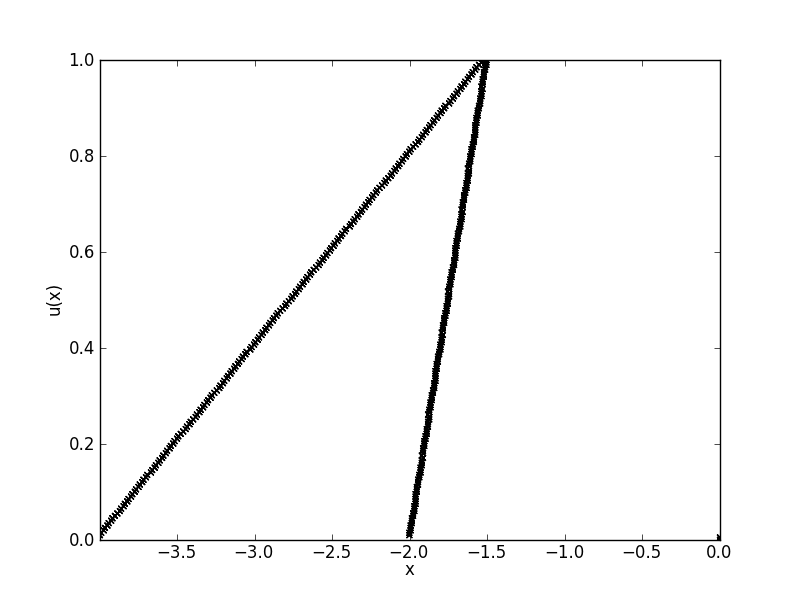
\includegraphics[width=0.15\textwidth]{graph19.png}
    }
    \subfigure[Multiplicação]{%
    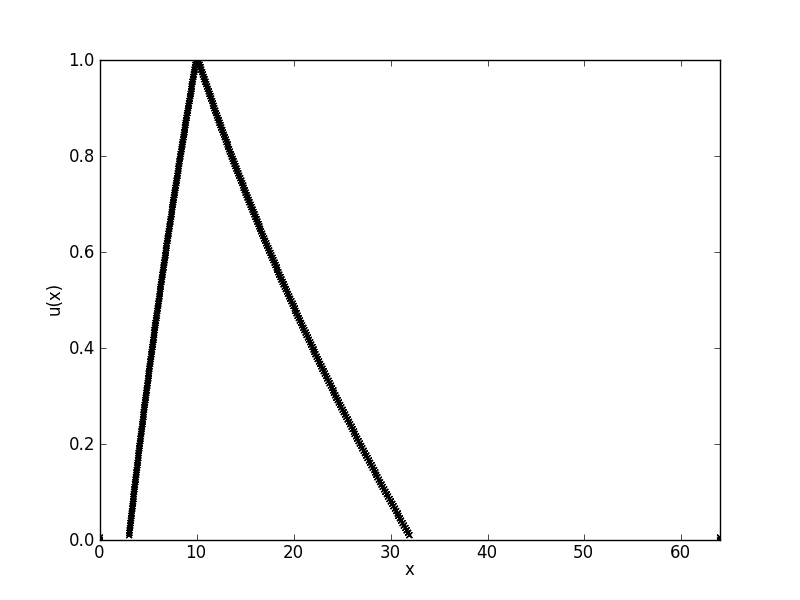
\includegraphics[width=0.15\textwidth]{graph20.png}
    }
    \subfigure[Divisão]{%
    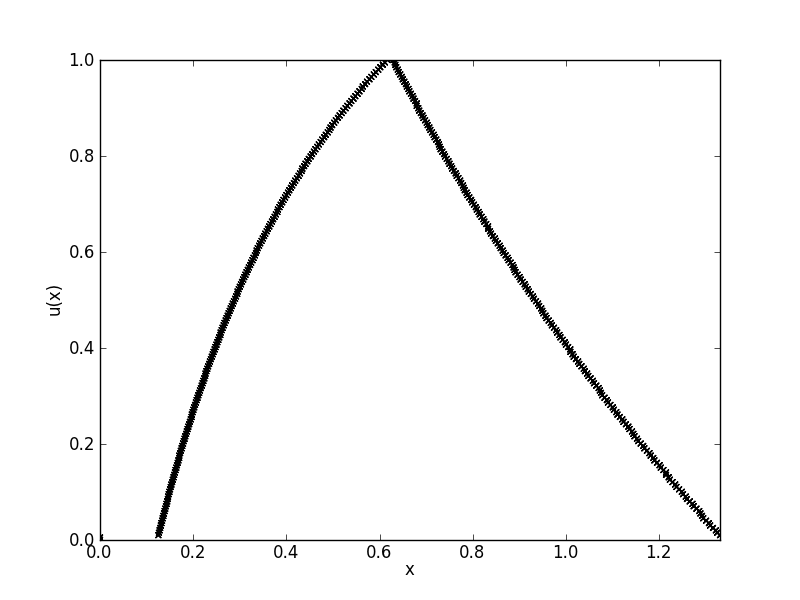
\includegraphics[width=0.15\textwidth]{graph21.png}
    }
    \subfigure[Mínimo]{%
    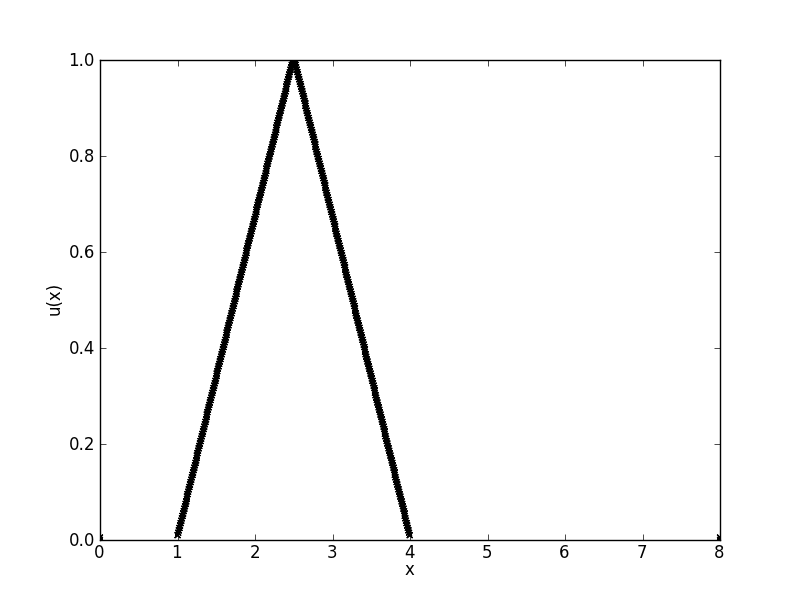
\includegraphics[width=0.15\textwidth]{graph22.png}
    }
    \subfigure[Máximo]{%
    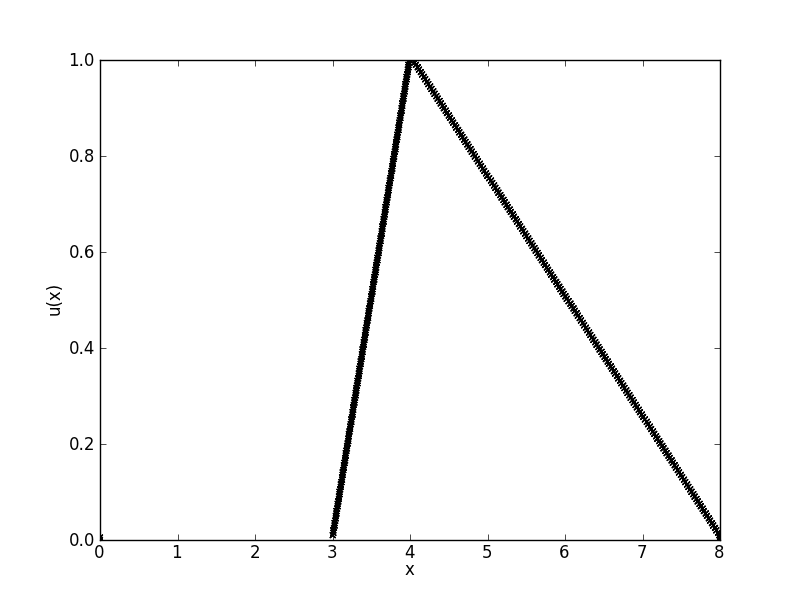
\includegraphics[width=0.15\textwidth]{graph23.png}
    }
\end{center}
\caption{$x_1$ = 2.5; $x_2$ = 4}
\end{figure}

\begin{figure}[h!]
\begin{center}
    \subfigure[Adição]{%
    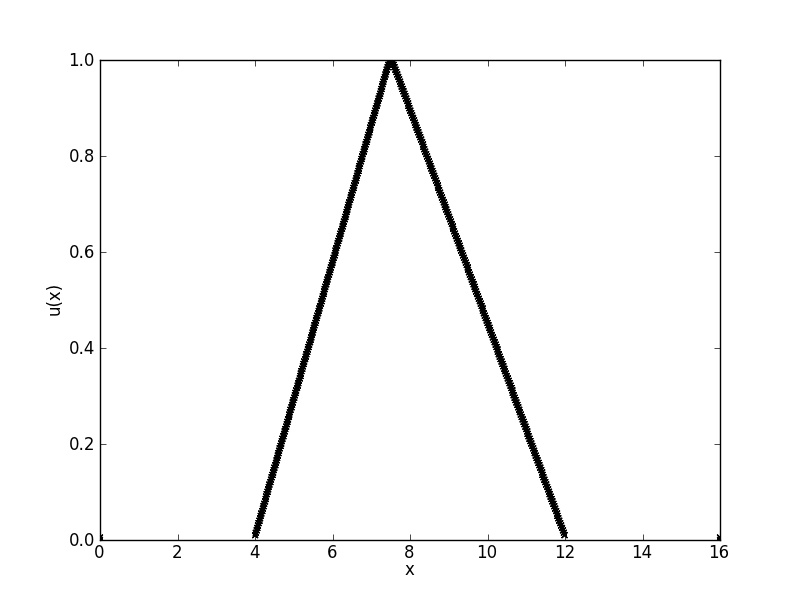
\includegraphics[width=0.15\textwidth]{graph24.png}
    }
    \subfigure[Subtração]{%
    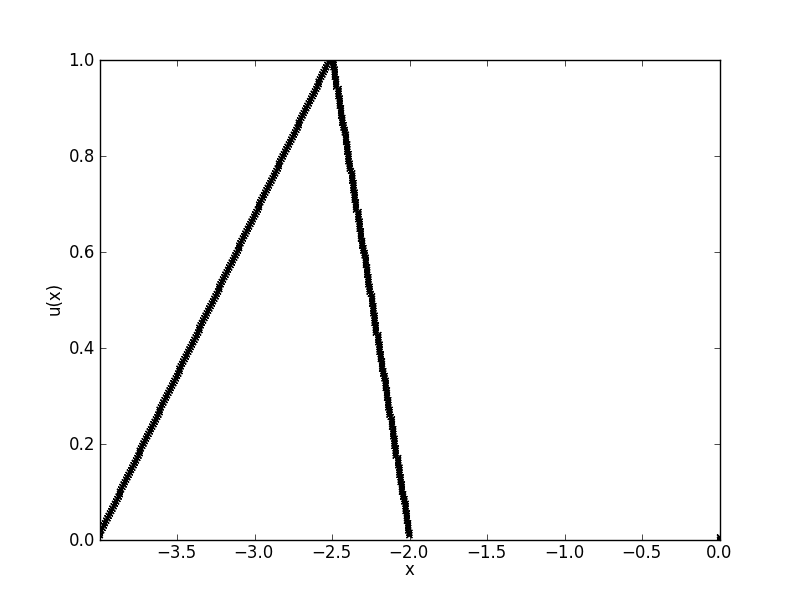
\includegraphics[width=0.15\textwidth]{graph25.png}
    }
    \subfigure[Multiplicação]{%
    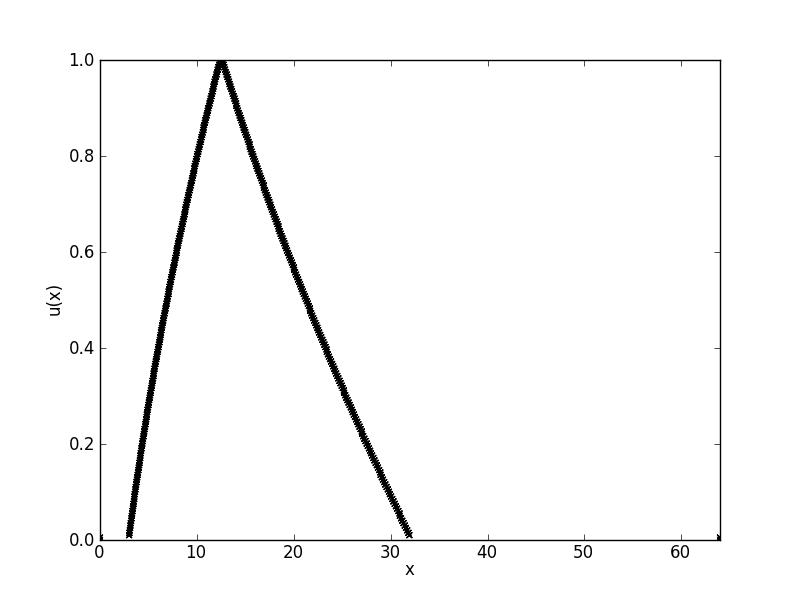
\includegraphics[width=0.15\textwidth]{graph26.png}
    }
    \subfigure[Divisão]{%
    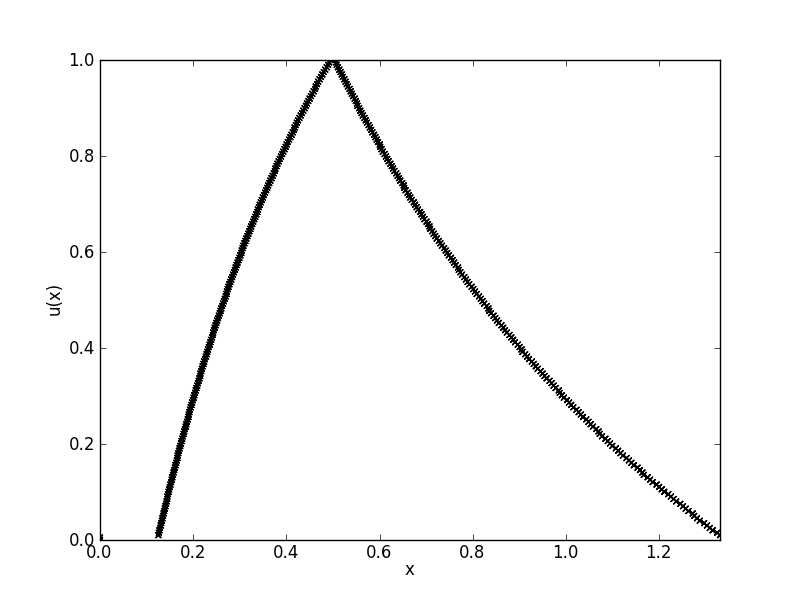
\includegraphics[width=0.15\textwidth]{graph27.png}
    }
    \subfigure[Mínimo]{%
    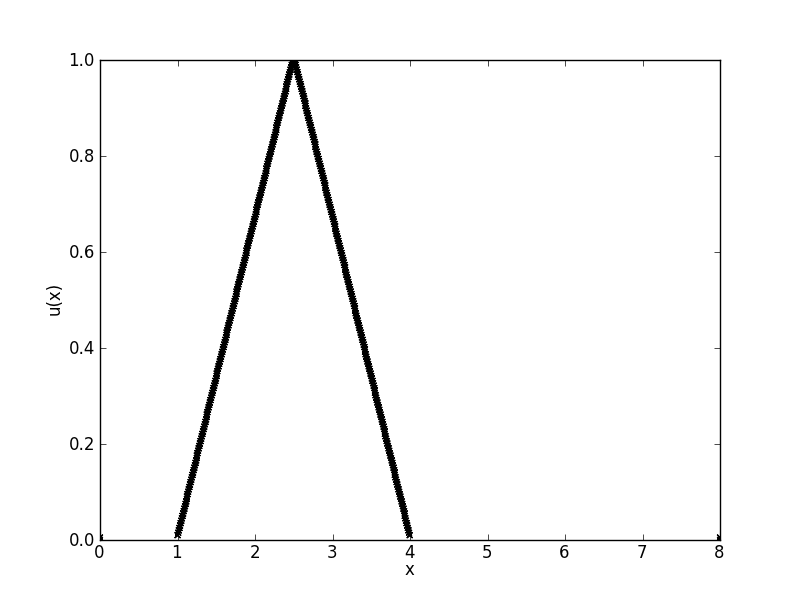
\includegraphics[width=0.15\textwidth]{graph28.png}
    }
    \subfigure[Máximo]{%
    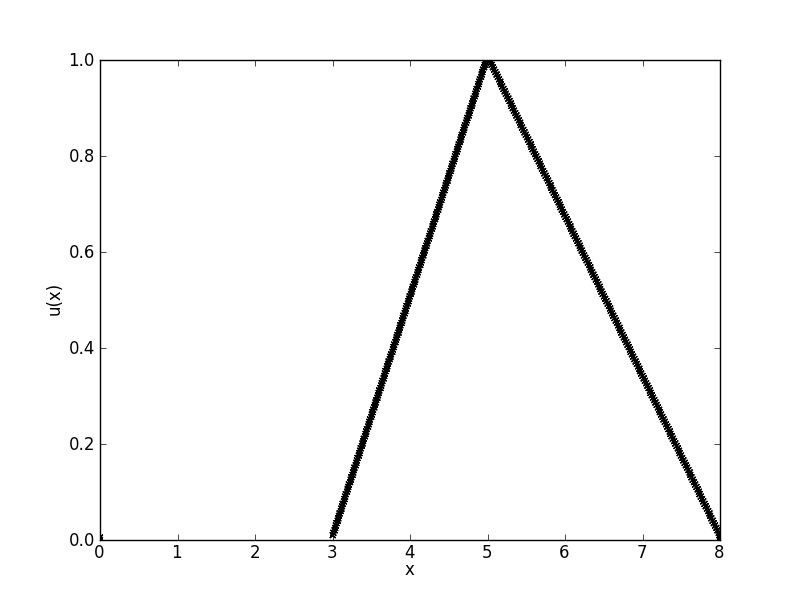
\includegraphics[width=0.15\textwidth]{graph29.png}
    }
\end{center}
\caption{$x_1$ = 2.5; $x_2$ = 5}
\end{figure}


\begin{figure}[h!]
\begin{center}
    \subfigure[Adição]{%
    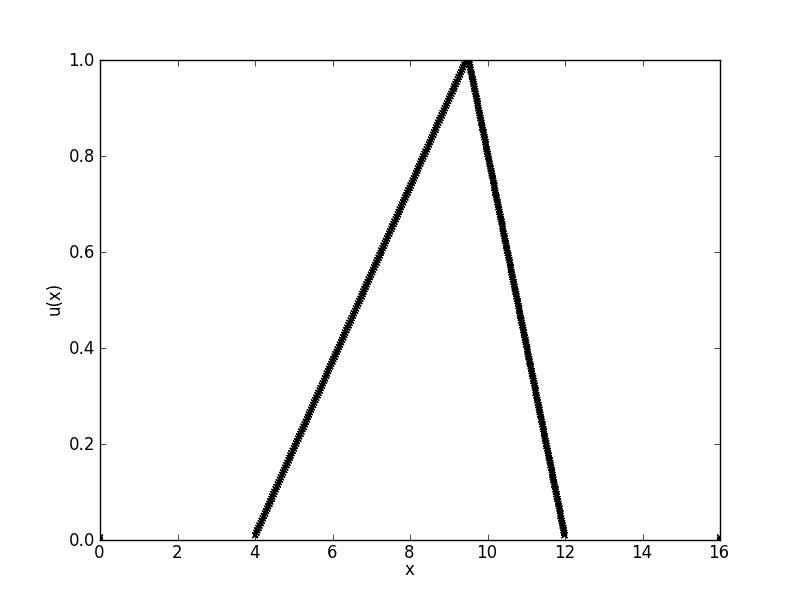
\includegraphics[width=0.15\textwidth]{graph30.png}
    }
    \subfigure[Subtração]{%
    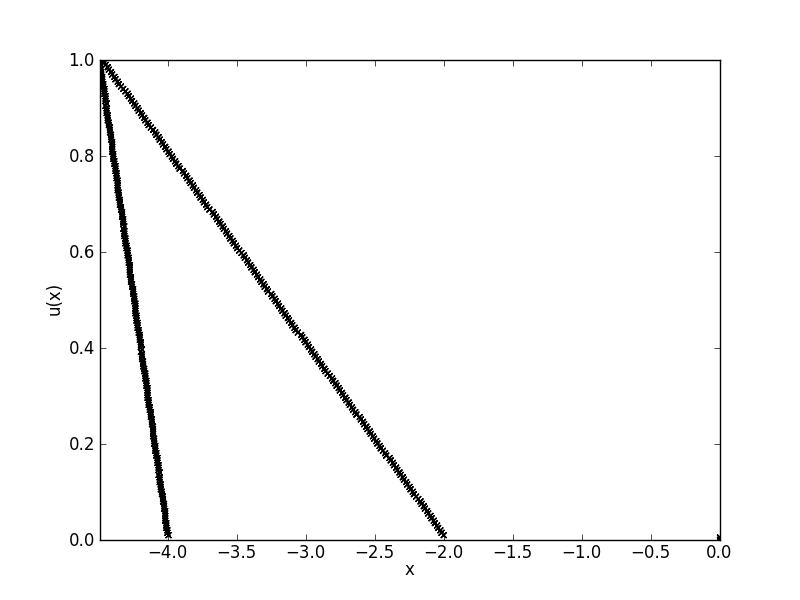
\includegraphics[width=0.15\textwidth]{graph31.png}
    }
    \subfigure[Multiplicação]{%
    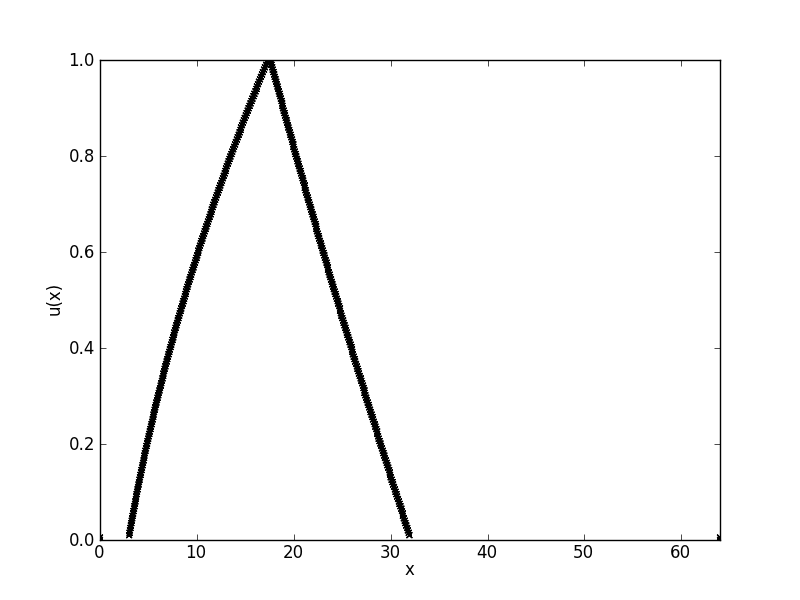
\includegraphics[width=0.15\textwidth]{graph32.png}
    }
    \subfigure[Divisão]{%
    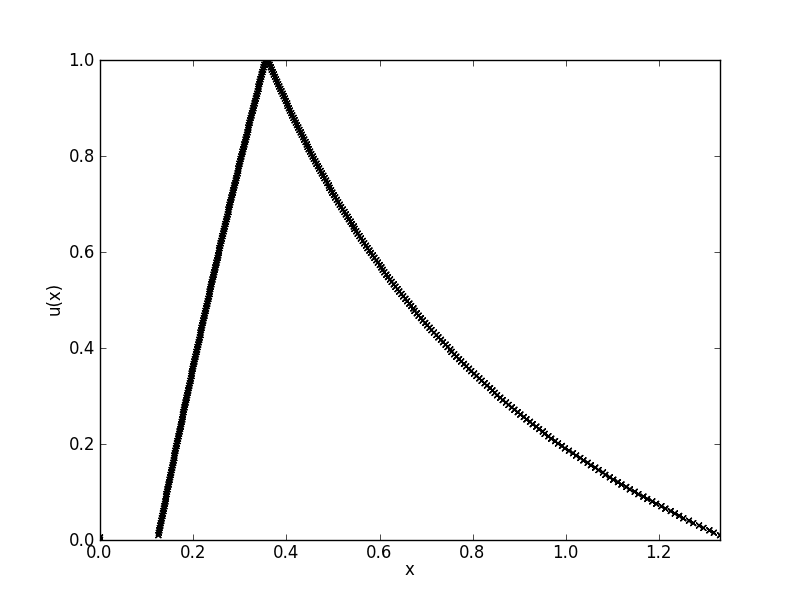
\includegraphics[width=0.15\textwidth]{graph33.png}
    }
    \subfigure[Mínimo]{%
    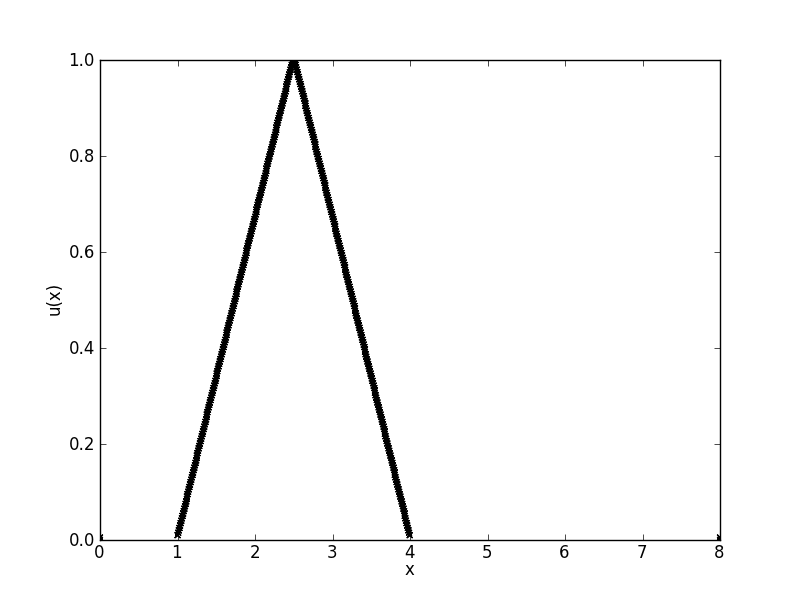
\includegraphics[width=0.15\textwidth]{graph34.png}
    }
    \subfigure[Máximo]{%
    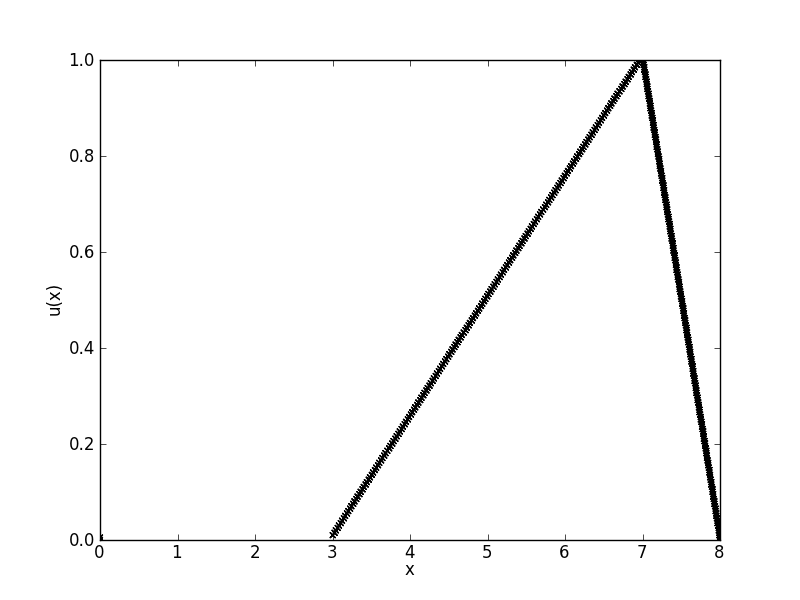
\includegraphics[width=0.15\textwidth]{graph35.png}
    }
\end{center}
\caption{$x_1$ = 2.5; $x_2$ = 7}
\end{figure}

\begin{figure}[h!]
\begin{center}
    \subfigure[Adição]{%
    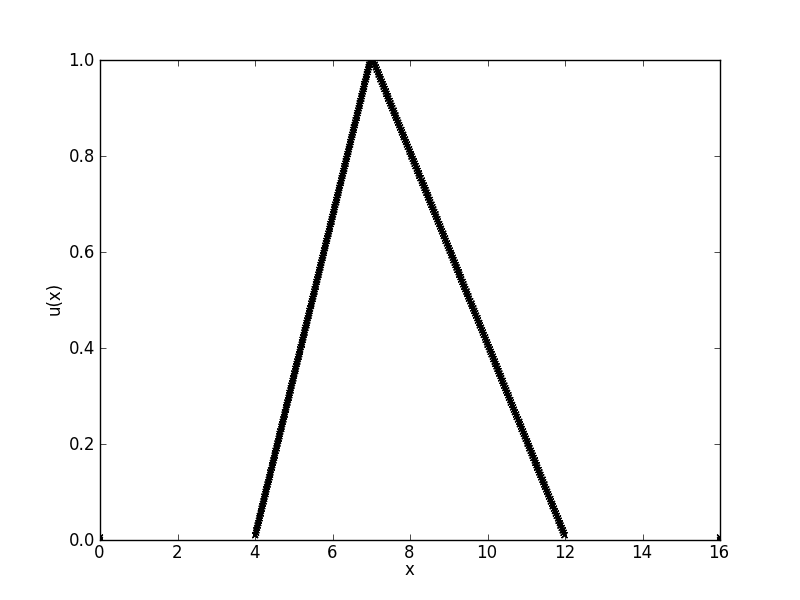
\includegraphics[width=0.15\textwidth]{graph36.png}
    }
    \subfigure[Subtração]{%
    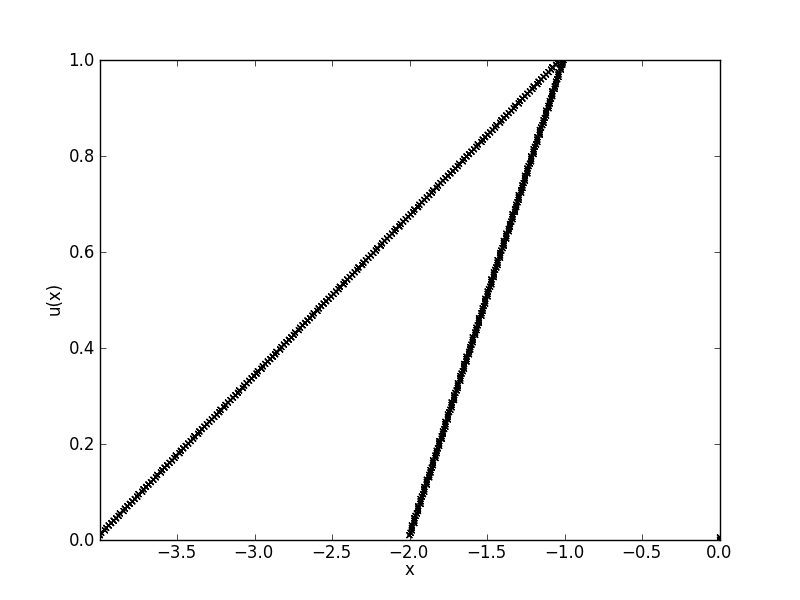
\includegraphics[width=0.15\textwidth]{graph37.png}
    }
    \subfigure[Multiplicação]{%
    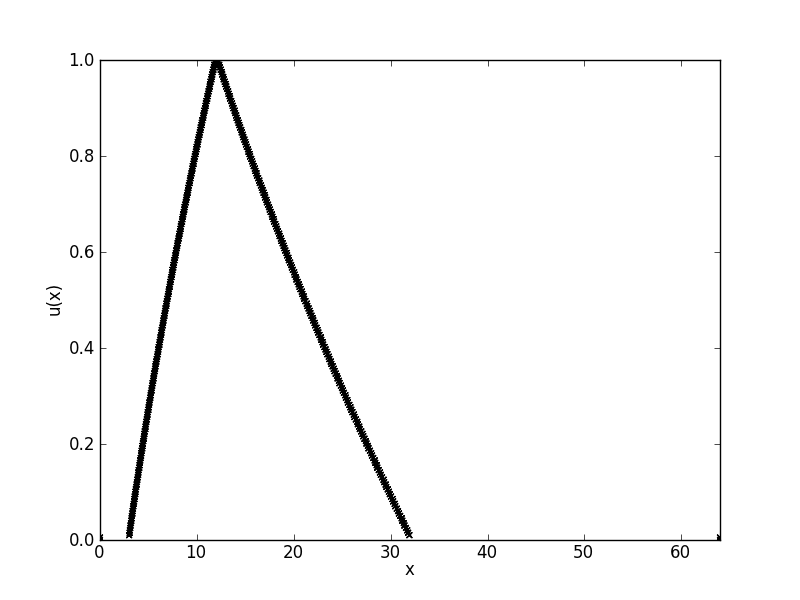
\includegraphics[width=0.15\textwidth]{graph38.png}
    }
    \subfigure[Divisão]{%
    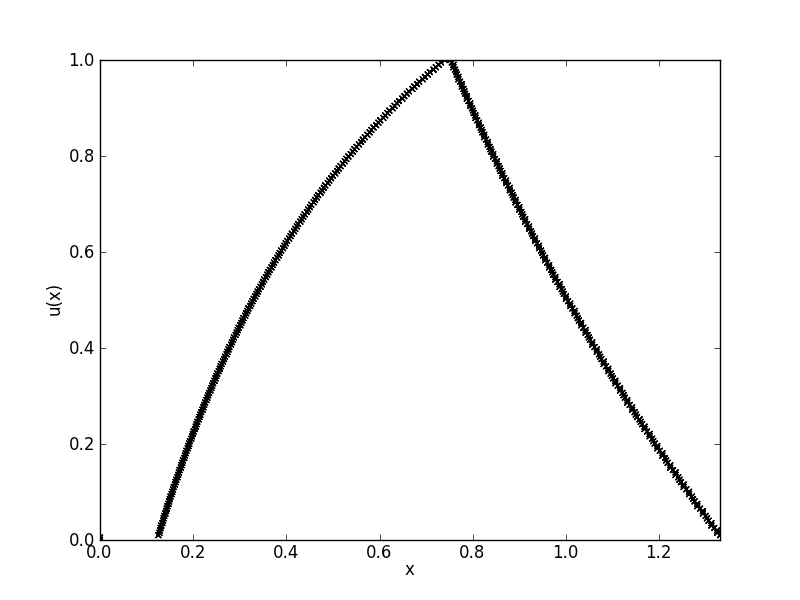
\includegraphics[width=0.15\textwidth]{graph39.png}
    }
    \subfigure[Mínimo]{%
    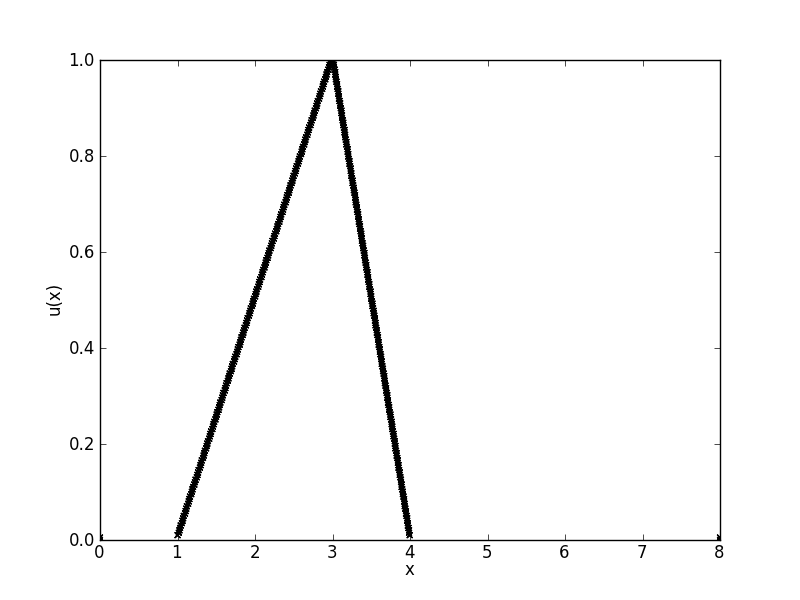
\includegraphics[width=0.15\textwidth]{graph40.png}
    }
    \subfigure[Máximo]{%
    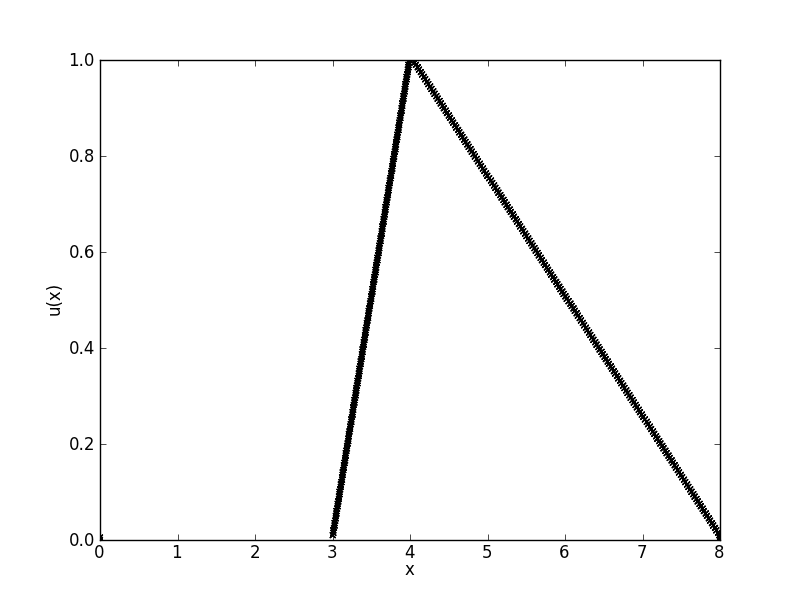
\includegraphics[width=0.15\textwidth]{graph41.png}
    }
\end{center}
\caption{$x_1$ = 3; $x_2$ = 4}
\end{figure}

\begin{figure}[h!]
\begin{center}
    \subfigure[Adição]{%
    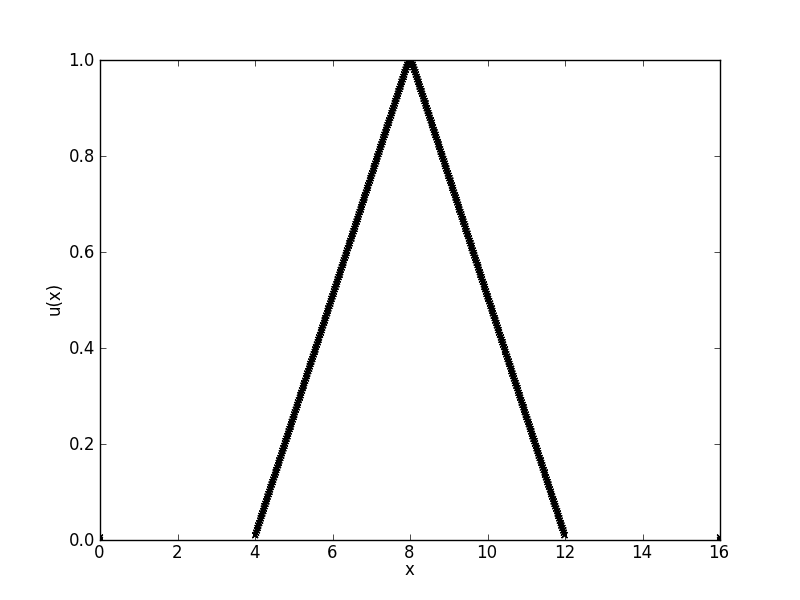
\includegraphics[width=0.15\textwidth]{graph42.png}
    }
    \subfigure[Subtração]{%
    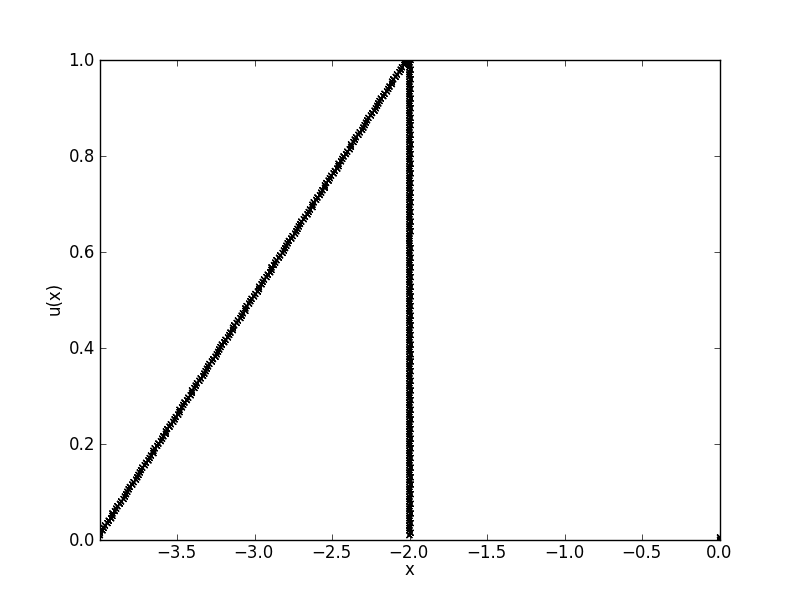
\includegraphics[width=0.15\textwidth]{graph43.png}
    }
    \subfigure[Multiplicação]{%
    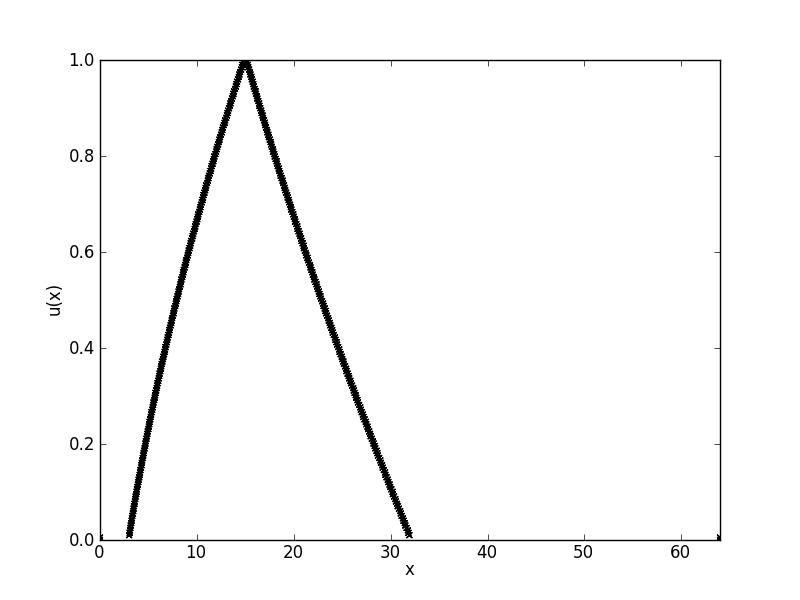
\includegraphics[width=0.15\textwidth]{graph44.png}
    }
    \subfigure[Divisão]{%
    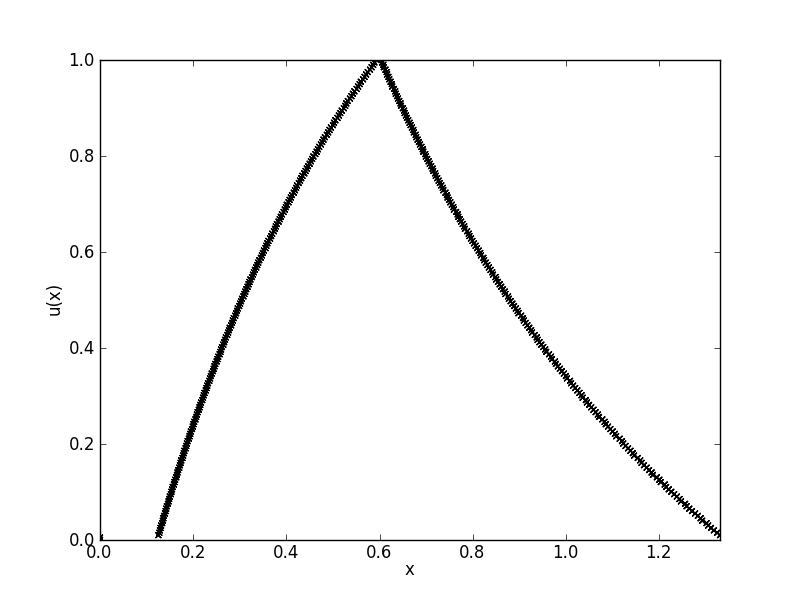
\includegraphics[width=0.15\textwidth]{graph45.png}
    }
    \subfigure[Mínimo]{%
    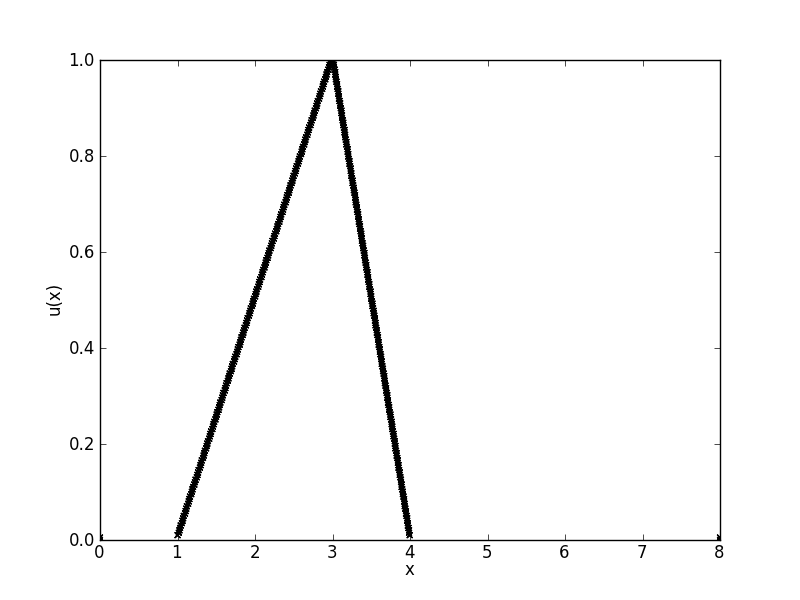
\includegraphics[width=0.15\textwidth]{graph46.png}
    }
    \subfigure[Máximo]{%
    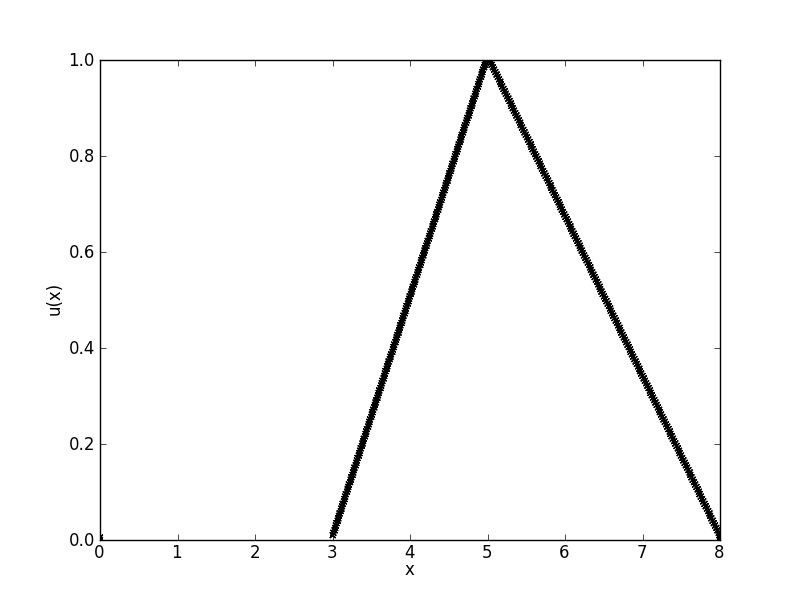
\includegraphics[width=0.15\textwidth]{graph47.png}
    }
\end{center}
\caption{$x_1$ = 3; $x_2$ = 5}
\end{figure}


\begin{figure}[h!]
\begin{center}
    \subfigure[Adição]{%
    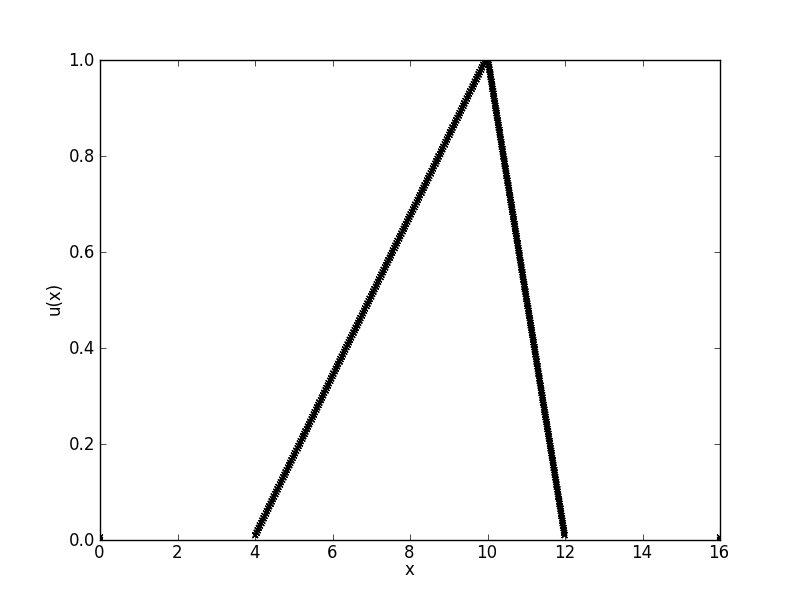
\includegraphics[width=0.15\textwidth]{graph48.png}
    }
    \subfigure[Subtração]{%
    \includegraphics[width=0.15\textwidth]{graph49.png}
    }
    \subfigure[Multiplicação]{%
    \includegraphics[width=0.15\textwidth]{graph50.png}
    }
    \subfigure[Divisão]{%
    \includegraphics[width=0.15\textwidth]{graph51.png}
    }
    \subfigure[Mínimo]{%
    \includegraphics[width=0.15\textwidth]{graph52.png}
    }
    \subfigure[Máximo]{%
    \includegraphics[width=0.15\textwidth]{graph53.png}
    }
\end{center}
\caption{$x_1$ = 3; $x_2$ = 7}
\end{figure}



\cleardoublepage
\lstset{basicstyle=\scriptsize}
\lstinputlisting[language=Python]{epc10.py}
%\lstinputlisting{resp.txt}

\end{document}
